\documentclass[11pt]{article}
\usepackage[margin=1in]{geometry}
\usepackage[T1]{fontenc}
\usepackage{lmodern}
\usepackage{microtype}
\usepackage{amsmath,amssymb}
\usepackage{booktabs}
\usepackage{graphicx}
\usepackage{xcolor}
\usepackage{enumitem}
\usepackage{fvextra}
\usepackage{tikz}
\usetikzlibrary{arrows.meta,positioning}
\usepackage[colorlinks=true,linkcolor=blue!50!black,citecolor=blue!50!black,urlcolor=blue!50!black]{hyperref}
\setlist{nosep,leftmargin=1.4em}
\hypersetup{pdftitle={Routing Edits: Reusing a Successor Circuit through Attention Weight Changes},pdfauthor={Yucheng Wang},pdfsubject={Mechanistic interpretability and circuit reuse}}
\newcommand{\head}[2]{L#1H#2}
\newcommand{\A}{\textsc{a}}

\title{Routing Edits: Reusing a Successor Circuit\\through Attention Weight Changes}
\author{Yucheng Wang\\[3pt]
\normalsize University of Wisconsin--Madison\\
\normalsize\texttt{ywang3574@wisc.edu}}
\date{}

\begin{document}
\maketitle

\begin{abstract}
A small language model can continue \texttt{c d e} with \texttt{f}, and it can retrieve \texttt{c} from a table. Can the two computations be connected, so that a lookup returns the successor of the retrieved value, without training on the combined task? We test whether the model's own successor computation can be reused by changing only where it reads its input. In Qwen3-0.6B-Base and Qwen3-1.7B-Base we locate an attention head involved in sequence succession and rewrite its query and key weights so that it attends to the retrieved value, leaving its value and output weights unchanged apart from a gain. A table containing \texttt{pine -> c}, queried with \texttt{pine ->}, now often elicits \texttt{d}: on fresh prompts, successor rates rise from 1--12\% to 46--69\% (0.6B) and from 6--25\% to 32--52\% (1.7B). Controls and output swaps show that the effect depends on the head's existing computation, not on the new attention alone. We then give a second language model circuit-level editing primitives; in all three runs it builds working edits, and in each it proposes a design we had not built, copying the successor circuit into another head. The direct edit has a measurable cost (14--17\% higher WikiText loss), and fine-tuning on composed examples works better. The result is a specific, causally tested case of reusing learned computation through a permanent weight change.
\end{abstract}

\section{Introduction}

Language models learn computations that they do not readily use together. Qwen3-0.6B-Base continues \texttt{e f g} with \texttt{h}, and given a short table it retrieves the value stored under a key. But on a lookup prompt it answers with the item \emph{after} the retrieved value on only 1--12\% of prompts. Neither computation is missing. What is missing is a connection between them: nothing routes the output of retrieval into the input of succession.

The usual way to create such a connection is to train on examples of the combined task, and that works well here (Section~\ref{sec:learning}). We ask whether the connection can instead be made directly in the weights: can a computation the model has already learned be reused by changing only where it receives its input? This is a question about \emph{weight-space programming} (WSP), the practice of reading a model's weights and activations and writing new weights directly instead of training on examples~\cite{sparks}. Our own first attempts at WSP followed the common pattern of asking a language model to propose small edits to improve a broad behaviour, and they produced no clear gain (Appendix~\ref{sec:negative}). Those failures pointed us toward a narrower target: a computation that is already localised in one component, whose input could be redirected.

Succession offers such a target. Many language models contain \emph{successor heads}, attention heads whose output maps a token to the next element of an ordinal sequence~\cite{gould2023successor}. An attention head separates, at least in part, where it reads (its query--key weights) from what it writes into the residual stream (its value--output weights)~\cite{elhage2021framework}. If the successor computation lives in the second part, then rewriting the first should send a new input through an unchanged computation.

We find a successor head at the same position, layer~21 head~6, in both Qwen3-0.6B-Base and Qwen3-1.7B-Base~\cite{qwen3}. Natively it reads the last item of a sequence. We replace its query and key weights in closed form so that, in a lookup prompt, it reads the queried value instead, and keep its value and output weights apart from a single gain (Figure~\ref{fig:schematic}). The edited model then answers lookups with the successor of the stored value on 46--69\% of fresh prompts in the 0.6B model and 32--52\% in the 1.7B model. The routing fit sees no successor targets; it is supervised only with the position of the queried value in ordinary-word lookups, although composed-task results were used to choose the gain.

\begin{figure}[t]
\centering
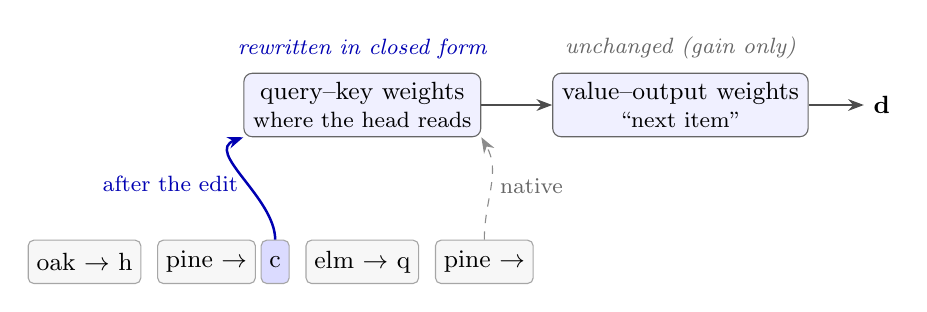
\begin{tikzpicture}[font=\small, tok/.style={draw=black!35, rounded corners=2pt, minimum height=5.5mm, inner xsep=3pt, fill=black!3},
  comp/.style={draw=black!60, rounded corners=3pt, minimum height=8mm, minimum width=24mm, align=center, fill=blue!6}, >={Stealth[length=2mm]}]
\node[tok] (a) {oak $\to$ h};
\node[tok, right=2mm of a] (b) {pine $\to$};
\node[tok, right=0.6mm of b, fill=blue!14] (v) {c};
\node[tok, right=2mm of v] (c) {elm $\to$ q};
\node[tok, right=2mm of c] (q) {pine $\to$};
\node[comp, above=13mm of c] (qk) {query--key weights\\[-1pt]{\footnotesize where the head reads}};
\node[comp, right=9mm of qk] (ov) {value--output weights\\[-1pt]{\footnotesize ``next item''}};
\node[right=7mm of ov] (out) {\textbf{d}};
\draw[->, blue!70!black, line width=0.9pt] (v.north) to[out=90, in=200] node[pos=0.45, left, font=\footnotesize, text=blue!70!black] {after the edit} (qk.south west);
\draw[->, black!45, dashed] (q.north) to[out=90, in=300] node[pos=0.5, right, font=\footnotesize, text=black!60] {native} (qk.south east);
\draw[->, black!70] (qk) -- (ov);
\draw[->, black!70] (ov) -- (out);
\node[above=0.5mm of qk, font=\footnotesize\itshape, text=blue!70!black] {rewritten in closed form};
\node[above=0.5mm of ov, font=\footnotesize\itshape, text=black!60] {unchanged (gain only)};
\end{tikzpicture}
\caption{The routing edit. A successor head natively reads the current token and writes a code for the next item. We rewrite its query and key weights so that, at the query position of a lookup prompt, it reads the queried value; its value and output weights are untouched. The model then answers the lookup with the successor of the stored value.}
\label{fig:schematic}
\end{figure}

The rest of the paper follows the questions this result raises. Is the effect really carried by the head's existing computation, or would any head with the new attention produce it? Controls and output swaps show that the head's own value--output circuit is necessary, and that attention alone is not enough (Section~\ref{sec:controls}). Does it transfer? It holds on unseen keys, unseen prompt formats, harder tables and a code-like assignment format (Sections~\ref{sec:main} and~\ref{sec:inc}). What does it break? The edit is global, and it raises language-modelling loss and disrupts the head's native role (Section~\ref{sec:gain}). Finally, having built the edit by hand, we asked whether another model could design it from circuit-level primitives and diagnostics. Claude Opus~5.5 assembled working edits in all three runs and, in each, proposed something we had not tried: transplanting the successor circuit into a different head so that the original can be left alone (Section~\ref{sec:opus}).

The routing is \emph{learned routing into an existing successor circuit}: a ridge regression and a singular value decomposition fitted to labelled positions, with no gradients but with supervision. We demonstrate one operation and one routing pattern, and the designer composes primitives that we wrote rather than deriving the construction itself. Within those bounds, the experiments give direct evidence that a pretrained computation can be reused through a permanent edit to where it reads.

\section{Related work}

Three lines of work bear on our question, and each leaves part of it open. Weight-space programming asks whether an editor can change a model by writing weights, but its successes so far repair or strengthen existing behaviour. Interpretability locates components such as successor heads and shows that they can be reused, mostly through activation interventions at inference time. Model editing makes permanent closed-form changes, but to stored knowledge rather than to how computations connect. What we test is whether a permanent edit to where a located pretrained computation reads can reuse that computation, and whether causal checks confirm that it was the computation itself that was reused.

\textbf{Can direct weight edits add behaviour?} The term weight-space programming and the first demonstrations are due to Takehi et al.~\cite{sparks}: a frontier reasoning model, acting through an agent harness, reads and edits the weights of small networks and repairs a degenerate looping behaviour in a small language model. They report that edits could remove a fault that hides an ability but could not add an ability the model lacked. Hu et al.~\cite{hu2026wsp} study sixteen editing trajectories on seven benchmarks and two model sizes and find gains from highly localised changes, uneven transfer, and several trajectories in which no reliable edit was found. Our own unsuccessful editing runs show similar limits (Appendix~\ref{sec:negative}). The routing edit is of a different kind. It does not repair or strengthen a behaviour; it joins a newly written routing circuit to a computation the model already has, and it is specified by a mechanism. Closed-form constructions in which a query--key circuit selects a position and an output--value circuit copies content have been written for toy networks trained or built from scratch~\cite{wspscratch,lindner2023tracr}. Tracr~\cite{lindner2023tracr} compiles whole programs into transformer weights. Our experiments study a related construction inside a pretrained model, where the computation being routed into was learned rather than written. We make no claim to exhaustive priority.

\textbf{Which components can be reused, and how?} The decomposition of attention into query--key routing and value--output computation is standard~\cite{elhage2021framework}, as are induction-style retrieval heads~\cite{olsson2022induction} and circuit analysis by activation patching~\cite{wang2023ioi}. Gould et al.~\cite{gould2023successor} identified successor heads and manipulated their representations, and Merullo et al.~\cite{merullo2024reuse} showed that circuit components are reused across tasks. These studies establish that the components exist and are shared. They do not test whether a component's input can be permanently redirected. Function vectors~\cite{todd2024function} are the closest precedent: their composition experiments combine item selection with word transformation through activation interventions. Our contribution is not the idea of composing selection and transformation but a specific permanent routing edit into a located successor-associated circuit, fitted with ordinary-word position labels, together with its causal evaluation.

\textbf{What can closed-form edits change?} ROME and MEMIT~\cite{meng2022rome,meng2023memit} write factual associations into MLP weights in closed form. QK Product Steering~\cite{tiwari2026qk} edits attention's query--key operator by suppressing singular modes and maps the change back to query weights, and TaRot~\cite{mbe2024} uses Bayesian optimisation to fit rotations of attention-head outputs. These methods change what a component stores or emphasises; we instead fit a new retrieval route into a selected computation. The tuned lens~\cite{belrose2023tuned} fits affine translators between layers, and our failed bridge constructions (Appendix~\ref{sec:negative}) explore related interfaces. Task arithmetic~\cite{ilharco2023task} and low-rank adaptation~\cite{hu2022lora} obtain weight changes from training, and serve as the natural alternative to closed-form construction.

\section{Setup}

\textbf{Models.} We use Qwen3-0.6B-Base (28 layers, width 1024) and Qwen3-1.7B-Base (28 layers, width 2048)~\cite{qwen3}. Both have 16 query heads of dimension 128 and 8 key/value groups (grouped-query attention~\cite{ainslie2023gqa}), query/key RMS normalisation, and rotary position embeddings~\cite{su2021roformer}. Unless stated otherwise, evaluation reads the next token's top-1 prediction over the full vocabulary in a single forward pass.

\textbf{Sequence prompts.} Native continuation of ordinal sequences, e.g.\ \texttt{e f g h} $\to$ \texttt{i}, in four layouts, over letters, number words, weekdays, months and ordinal words. These prompts locate the successor head; separate small sequence sets are also used to probe collateral effects.

\textbf{Lookup prompts.} Tables of three to five key--value lines followed by a query for one key:
\begin{center}\texttt{oak -> h \quad pine -> c \quad elm -> q \quad pine ->}\end{center}
(one pair per line). The \emph{lookup} answer is the stored value (\texttt{c}); the \emph{successor} answer is the next item after it (\texttt{d}). For ordinal value types we reject tables in which two values are adjacent or in which the correct successor appears as another value; Section~\ref{sec:controls} removes these restrictions. Keys are common nouns. Two further formats, \texttt{k:~v} and \texttt{k~=~v}, are used only for testing.

\textbf{Metric.} The \emph{successor rate} is the fraction of prompts whose top-1 token matches the first token of the successor of the queried value. Targets are tokenised with a leading space for the lookup task. The generator filters stored ordinal values to single-token items, but the metric itself checks only the first answer token; it does not verify a complete generated string. Weekdays and months wrap cyclically, and terminal items without a successor in the other lists are rejected. We also report the lookup rate, language-model loss on a fixed WikiText sample, and lookup accuracy on tables with ordinary-word values. The digit task uses assignment-context tokenisation; its two-digit exact-match check is reported separately.

\section{Method}\label{sec:method}

\subsection{Locating the operation head}\label{sec:locate}

Redirecting a computation requires a component whose output, on its own, determines the answer. We therefore look for a head with that property on native sequence prompts before touching the lookup task. We fix the following rule before applying it to any model other than the one it was developed on. (i)~On sequence prompts, set each head's output at the final position to zero and rank heads by the drop in the logit margin between the correct next item and the item after it. (ii)~For the six highest-ranked heads, replace the head's output at the final position by its own value vector taken from the prompt that ends one item later, and measure how often the model then answers two steps ahead. (iii)~Select the head with the highest two-step rate. Lookup prompts are not used.

On Qwen3-0.6B-Base the rule selects \head{21}{6} (two-step rate 0.92; the next candidate reaches 0.34). On Qwen3-1.7B-Base it also selects \head{21}{6} (0.97; next candidate 0.32). An earlier search that used only the weights of the 0.6B model (reading each head's output--value map through the unembedding) had ranked the same head first. We refer to the selected head as \A\ (Figure~\ref{fig:locate}).

\begin{figure}[t]
\centering
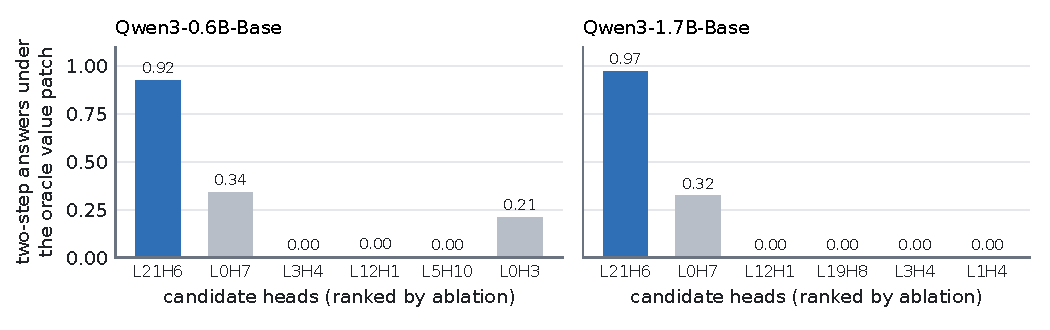
\includegraphics[width=\linewidth]{figures/locate.pdf}
\caption{Step (ii) of the locating rule on both models. For each of the six heads ranked highest by ablation, the head's output at the final position of a sequence prompt is replaced by its value vector from the prompt ending one item later. One head, at the same position in both models, makes the model answer two steps ahead.}
\label{fig:locate}
\end{figure}

The oracle in step (ii) is the fact the edit relies on: if \A's output is the value vector of a position that holds item $x$, the rest of the network produces the successor of $x$. The remaining task is to make \A\ read from the right position.

\subsection{The attention programme}\label{sec:program}

Let $x_s \in \mathbb{R}^d$ be the normalised residual stream entering layer 21 at position $s$. For a lookup prompt let $f$ be this vector at the final position and $v$ the vector at the position of the queried value token. We want \A's attention from the final position to concentrate on that position. Over a set of lookup prompts whose values are ordinary words we accumulate
\begin{equation}
C_{ff} = \mathbb{E}\!\left[f f^{\top}\right],\qquad
C_{kk} = \mathbb{E}_s\!\left[x_s x_s^{\top}\right],\qquad
X = \mathbb{E}\!\left[f\,(v - \bar{x}_{\neg v})^{\top}\right],
\end{equation}
where $\bar{x}_{\neg v}$ is the mean over the other positions of the same prompt, and form the whitened bilinear map
\begin{equation}
B = \left(C_{ff} + \lambda_f I\right)^{-1} X \left(C_{kk} + \lambda_k I\right)^{-1},\qquad \lambda_f = \lambda\,\tfrac{\operatorname{tr} C_{ff}}{d},\ \ \lambda_k = \lambda\,\tfrac{\operatorname{tr} C_{kk}}{d}.
\end{equation}
With the singular value decomposition $B = U S V^{\top}$ truncated to rank $r = 64$, the query rows are $W_Q = S_r^{1/2} U_r^{\top}$ and the key rows are $W_K = S_r^{1/2} V_r^{\top}$, so that $(W_Q f)^{\top}(W_K x_s) = f^{\top} B_r\, x_s$. In words, $X$ records which directions in the final position co-occur with which directions at the queried value, relative to the other positions in the prompt; whitening removes directions that are large everywhere; and the factorisation turns this score into query and key weights for one head. Because the fit uses ordinary-word values, it learns \emph{where} the value sits, not what the value is.

\textbf{Installation.} Rotary embeddings rotate dimension pairs $(j, j{+}64)$ of each query and key by an angle proportional to position times $\theta^{-j/64}$ with $\theta = 10^6$. We write the 64 rows into pairs with $j \ge 32$, whose rotation per position is at most $10^{-3}$ radians, and set \A's other query and key rows to zero. This reduces positional variation over the short tables tested here; rotation still accumulates with distance, so this is not evidence for long-context routing.

The bilinear identity above describes the projections before query/key normalisation and rotary embeddings. More precisely, let $\tilde q=E W_Q f$ and $\tilde k_s=E W_K x_s$, where $E$ places the rows in the selected 128-dimensional coordinates. The installed pre-softmax score is
\begin{equation}
 a_s=\frac{[R_t D_q\tilde q]^{\top}[R_s D_k\tilde k_s]}
 {\sqrt{128}\,\rho(\tilde q)\rho(\tilde k_s)},\qquad
 \rho(z)=\sqrt{\|z\|_2^2/128+\epsilon},
\end{equation}
where $t$ is the query position, $R$ is the rotary transform, and $D_q,D_k$ contain the pretrained per-coordinate RMSNorm gains. These gains and the normalisation epsilon are retained; the edit changes only the projection rows and the output gain. Thus the actual score includes both learned coordinate scaling and input-dependent normalisation. We validate it using the attention it produces. Head~6 shares its key group with head~7, whose keys also change; removing head~7 does not materially change the result (Section~\ref{sec:controls}).

\textbf{Choice of $\lambda$ and gain.} $\lambda \in \{10^{-3},10^{-2},10^{-1},1\}$ is chosen by \A's mean attention on the queried value in held-out ordinary-word lookups ($\lambda = 1$ for both models). \A's output projection is multiplied by a gain $g$. The gain was chosen as $g=3$ after inspecting results on the 0.6B model's first evaluation prompts; it was then frozen, and all confirmation results use prompts generated afterwards. For the 1.7B model nothing was chosen on its data except $\lambda$ by the stated rule.

\textbf{Fitting, selection and confirmation.} The routing fit uses 1{,}500 lookup prompts with ordinary-word values and the queried position marked. It includes no ordinal-value examples or successor targets. Sequence prompts are used earlier to locate the head, and composed-task performance is used later to choose the gain. Confirmation then evaluates the frozen edit on fresh prompts. Throughout, value types described as unseen are unseen during routing fitting, rather than throughout development. The fit is supervised linear algebra; it uses no gradients.

\section{Results}\label{sec:results}

\subsection{Main result and replication}\label{sec:main}

The first question is whether the rewritten head reads where we intended. It does. The programmed attention reaches the queried value: \A's mean attention on it is 0.75 on held-out ordinary-word lookups and 0.73--0.88 on prompts with ordinal values (0.01 natively) in the 0.6B model, and 0.73 and 0.51--0.82 in the 1.7B model.

The second is whether the redirected head now produces the composed answer. Table~\ref{tab:main} and Figure~\ref{fig:main} give the confirmation results: 400 fresh prompts per cell, key words never used in fitting, and two prompt formats never used in fitting. The successor rate rises in all 30 cells. On the 0.6B model it reaches 0.46--0.69 in the fitted format (from 0.01--0.12) and 0.45--0.69 in the unseen formats. On the 1.7B model, with the procedure frozen, it reaches 0.32--0.52 (from 0.06--0.25) and 0.29--0.55 in the unseen formats. The effect is smaller on the larger model, whose native successor rate is higher and whose native lookup in these formats is less reliable.

\begin{figure}[t]
\centering
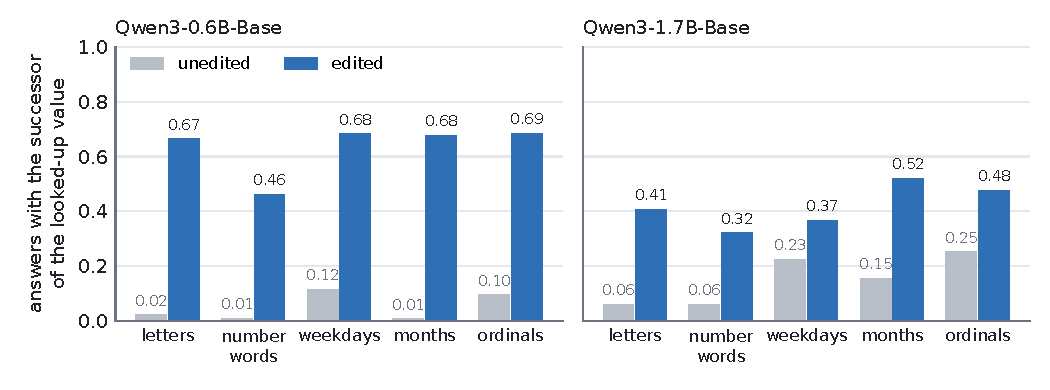
\includegraphics[width=\linewidth]{figures/main_result.pdf}
\caption{Successor rate before and after the routing edit on fresh lookup prompts with unseen key words (fitted format, 400 prompts per bar). The edit is fitted on ordinary-word lookups only.}
\label{fig:main}
\end{figure}

\begin{table}[t]
\centering\small
\resizebox{\linewidth}{!}{\begin{tabular}{llcccccc}
\toprule
 & & \multicolumn{3}{c}{Qwen3-0.6B-Base} & \multicolumn{3}{c}{Qwen3-1.7B-Base} \\
\cmidrule(lr){3-5}\cmidrule(lr){6-8}
Format & Values & Unedited & Edited & W / L & Unedited & Edited & W / L \\
\midrule
$k \rightarrow v$ & Letters & .02 & \textbf{.67} & 261 / 4 & .06 & \textbf{.41} & 144 / 5 \\
 & Number words & .01 & \textbf{.46} & 182 / 1 & .06 & \textbf{.32} & 116 / 11 \\
 & Weekdays & .12 & \textbf{.68} & 237 / 10 & .23 & \textbf{.37} & 96 / 39 \\
 & Months & .01 & \textbf{.68} & 268 / 0 & .15 & \textbf{.52} & 175 / 29 \\
 & Ordinals & .10 & \textbf{.69} & 254 / 18 & .25 & \textbf{.48} & 145 / 55 \\
\midrule
$k$: $v$ & Letters & .02 & \textbf{.59} & 231 / 0 & .04 & \textbf{.47} & 179 / 8 \\
 & Number words & .07 & \textbf{.57} & 211 / 12 & .04 & \textbf{.41} & 154 / 5 \\
 & Weekdays & .22 & \textbf{.61} & 192 / 34 & .16 & \textbf{.49} & 162 / 31 \\
 & Months & .05 & \textbf{.62} & 235 / 7 & .14 & \textbf{.51} & 177 / 28 \\
 & Ordinals & .21 & \textbf{.65} & 216 / 40 & .23 & \textbf{.51} & 171 / 63 \\
\midrule
$k = v$ & Letters & .05 & \textbf{.49} & 184 / 9 & .02 & \textbf{.42} & 164 / 3 \\
 & Number words & .08 & \textbf{.45} & 166 / 18 & .04 & \textbf{.29} & 107 / 4 \\
 & Weekdays & .30 & \textbf{.59} & 169 / 53 & .21 & \textbf{.48} & 133 / 27 \\
 & Months & .09 & \textbf{.69} & 254 / 15 & .08 & \textbf{.55} & 199 / 11 \\
 & Ordinals & .24 & \textbf{.60} & 182 / 41 & .26 & \textbf{.41} & 118 / 58 \\
\bottomrule
\end{tabular}
}
\caption{Successor rate, unedited and edited, on confirmation prompts (400 per cell; unseen key words). W / L: prompts that became successor answers / prompts that stopped being successor answers. The $k \rightarrow v$ format was used for fitting (with ordinary-word values); the other two formats were not.}
\label{tab:main}
\end{table}

\subsection{Controls and causal checks}\label{sec:controls}

A rise in successor answers could have other causes: the new attention pattern itself, the extra output gain, or some side effect of the edit on the shared key group. The controls separate these possibilities.

\textbf{The behaviour is carried by \A.} With the edit in place, zeroing \A's output returns the successor rate to the unedited level, and replacing \A's output by the one computed on a different prompt makes the model answer with \emph{that} prompt's successor (Table~\ref{tab:causal}). Restricting the swap to donors that query a different value gives 0.41--0.67 for the donor's successor against 0.00--0.05 for the prompt's own (Table~\ref{tab:cf}).

\begin{table}[t]
\centering\small
\resizebox{\linewidth}{!}{\begin{tabular}{lcccccc}
\toprule
 & \multicolumn{3}{c}{Qwen3-0.6B-Base} & \multicolumn{3}{c}{Qwen3-1.7B-Base} \\
\cmidrule(lr){2-4}\cmidrule(lr){5-7}
Values & Head removed & Donor's succ. & Own succ. & Head removed & Donor's succ. & Own succ. \\
\midrule
Letters & .00 & .72 & .03 & .01 & .36 & .03 \\
Number words & .01 & .38 & .03 & .01 & .25 & .02 \\
Weekdays & .07 & .63 & .15 & .08 & .36 & .11 \\
Months & .01 & .59 & .07 & .03 & .47 & .07 \\
Ordinals & .04 & .57 & .11 & .12 & .43 & .11 \\
\bottomrule
\end{tabular}
}
\caption{Interventions with the edit in place (fitted format, unseen keys, 400 prompts per cell). ``Head removed'': successor rate when \A's output is zeroed. ``Donor's succ.''/``Own succ.'': \A's output is taken from another prompt of the same value type.}
\label{tab:causal}
\end{table}

\textbf{The attention weights alone are not enough.} Installing the same query and key rows in six other heads of layer 21, each keeping its own value and output weights and the same gain, produces the same attention on the queried value (0.78) and does not reproduce the effect: successor rates stay at 0.00--0.09, except for one head at 0.19 on weekdays, close to the unedited rate for that type (Table~\ref{tab:controls}, Figure~\ref{fig:controls}). Conversely, the programmed attention with another head's output projection, a gain without the programmed attention, an attention programme fitted to a random other position, and random query/key rows with the same singular values, rank and placement all stay near the unedited rate. Removing head~7, which shares \A's rewritten keys, changes nothing.

\begin{table}[t]
\centering\small
\resizebox{\linewidth}{!}{\begin{tabular}{lccccc}
\toprule
Condition & Letters & Number words & Weekdays & Months & Ordinals \\
\midrule
Unedited model & .02 & .02 & .14 & .04 & .09 \\
Edit (successor head, gain 3) & .60 & .53 & .66 & .64 & .69 \\
\midrule
Same attention, six other heads (mean) & .01 & .01 & .05 & .02 & .03 \\
Same attention, six other heads (max) & .02 & .03 & .19 & .04 & .09 \\
Attention fitted to a wrong position & .00 & .01 & .09 & .02 & .06 \\
Random attention, matched spectrum (mean of 3) & .03 & .01 & .12 & .02 & .07 \\
Gain only, native attention & .05 & .04 & .23 & .09 & .10 \\
Edit with another head's output projection & .03 & .04 & .08 & .02 & .03 \\
Edit, neighbour head (shared keys) removed & .61 & .52 & .67 & .66 & .69 \\
\bottomrule
\end{tabular}
}
\caption{Successor rate under controls, Qwen3-0.6B-Base, gain 3, 300 fresh prompts per value type. The first two rows are the reference; all others are controls except the last, which tests the shared key group. The wrong-position, gain-only and alternative-output-projection rows use the initial evaluation prompts; the remaining rows use a separate controls evaluation. Each set contains 300 prompts per value type.}
\label{tab:controls}
\end{table}

\begin{figure}[t]
\centering
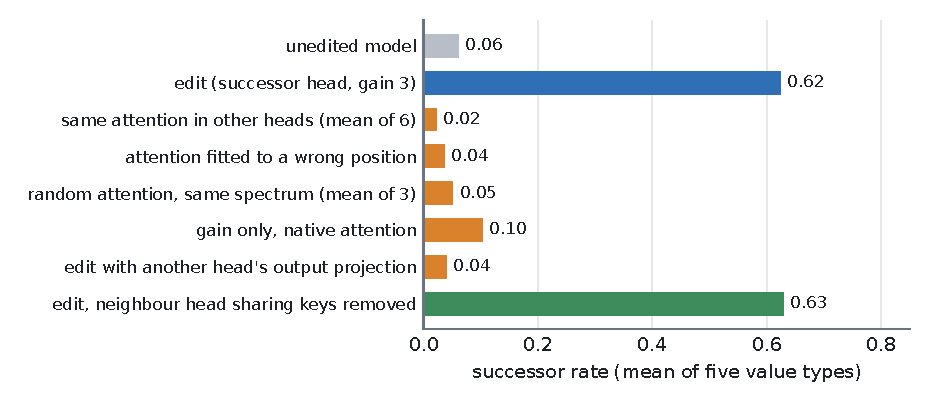
\includegraphics[width=0.86\linewidth]{figures/controls.pdf}
\caption{Controls from Table~\ref{tab:controls}, averaged over value types.}
\label{fig:controls}
\end{figure}

\textbf{Harder prompts.} The effect holds when adjacent ordinal values are allowed, when the correct successor is present in the table as a distractor, and for eight-row tables (Table~\ref{tab:cf}).

\begin{table}[t]
\centering\small
\resizebox{\linewidth}{!}{\begin{tabular}{lccccc}
\toprule
Prompt variant & Letters & Number words & Weekdays & Months & Ordinals \\
\midrule
Adjacent values allowed & .02$\,\to\,$.65 & .02$\,\to\,$.56 & .10$\,\to\,$.74 & .02$\,\to\,$.72 & .10$\,\to\,$.80 \\
Correct successor present as a distractor & .06$\,\to\,$.66 & .05$\,\to\,$.65 & .14$\,\to\,$.71 & .16$\,\to\,$.69 & .10$\,\to\,$.78 \\
Eight-row tables & .01$\,\to\,$.62 & .00$\,\to\,$.56 & -- & .02$\,\to\,$.76 & .07$\,\to\,$.78 \\
\midrule
Swap, donor value differs: donor's successor & .67 & .41 & .66 & .61 & .56 \\
Swap, donor value differs: own successor & .01 & .03 & .05 & .00 & .01 \\
\bottomrule
\end{tabular}
}
\caption{Qwen3-0.6B-Base. Top: successor rate, unedited $\to$ edited, on prompt variants that the standard generator excludes (300 prompts each; weekdays have too few values for eight-row tables). Bottom: output swaps counted only when the donor prompt queries a different value.}
\label{tab:cf}
\end{table}

\subsection{Variable lookup and increment}\label{sec:inc}

If the edit reuses a general successor computation rather than something specific to word lists, it should also work when the values are digits in a code-like format. The same procedure applies to a code-like format with digit values: assignments \texttt{x=3}, \texttt{total=7}, \texttt{n=5}, then \texttt{total=}. The attention programme is fitted on assignments whose values are ordinary words; digits are never seen. Table~\ref{tab:inc} shows that the edited models answer with the incremented value in 60\% (0.6B) and 42\% (1.7B) of prompts at gain 3, against 7\% and 3\% unedited, with controls at 2--17\%. In the 0.6B model the edited increment rate exceeds the unedited model's rate of copying the value (34\%); these are output accuracies and do not by themselves establish that retrieval became more accurate. The edit acts on one token: for two-digit values the exact-match increment rate is 0.04.

\begin{table}[t]
\centering\small
\begin{tabular}{lcccc}
\toprule
 & \multicolumn{2}{c}{Qwen3-0.6B-Base} & \multicolumn{2}{c}{Qwen3-1.7B-Base} \\
\cmidrule(lr){2-3}\cmidrule(lr){4-5}
Condition & $v{+}1$ & $v$ & $v{+}1$ & $v$ \\
\midrule
Unedited model & .07 & .34 & .03 & .40 \\
Edit, gain 1 & .36 & .23 & .26 & .28 \\
Edit, gain 2 & .53 & .17 & .39 & .21 \\
Edit, gain 3 & .60 & .14 & .42 & .20 \\
Edit, gain 4 & .66 & .11 & .47 & .18 \\
\midrule
Edit (gain 3), successor head removed & .03 & .39 & .02 & .43 \\
Attention fitted to a wrong position & .06 & .32 & .05 & .33 \\
Gain only, native attention & .17 & .33 & .05 & .40 \\
Edit with another head's output projection & .04 & .27 & .09 & .28 \\
\bottomrule
\end{tabular}

\caption{Single-digit assignments (600 prompts): fraction answered with the incremented value $v{+}1$ and with the stored value $v$.}
\label{tab:inc}
\end{table}

\subsection{The gain and the cost of the edit}\label{sec:gain}

A permanent edit to a head that the model already uses will cost something. We measure that cost against the one free parameter, the output gain. Figure~\ref{fig:gain} varies the gain on the 0.6B model. The mean logit margin between the successor and the looked-up value grows steadily with the gain and crosses zero between gains 0.5 and 3 depending on the value type, which is consistent with \A's vote for the successor having to out-vote the unchanged pathways that copy the value. We have not isolated those pathways, and other explanations (effects on downstream normalisation or nonlinearities) are not excluded.

The edit has three costs. Rewriting \A's attention removes its native role, and plain sequence continuation degrades. With the programmed attention installed and \A's output zeroed (gain 0), WikiText loss rises by 2.6\%; this intervention also includes the change to the shared key rows, so it is not a measurement of the attention rewrite alone. The gain adds further damage: loss rises by 4\%, 9\%, 17\% and 26\% at gains 1--4 on the 0.6B model (14\% at gain 3 on the 1.7B model). And the edit is global: lookups with ordinary-word values fall from 0.64 to 0.54 at gain 3.

\begin{figure}[t]
\centering
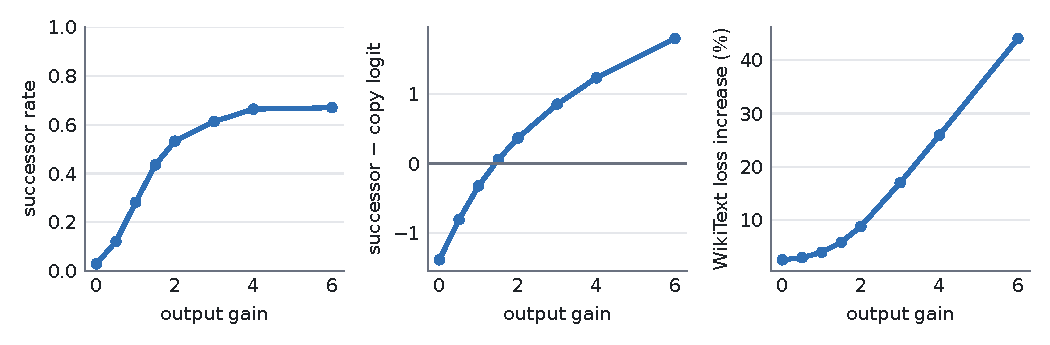
\includegraphics[width=\linewidth]{figures/gain.pdf}
\caption{Qwen3-0.6B-Base, closed-form edit, as a function of the gain on \A's output projection: successor rate and successor-minus-copy logit margin (means over five value types), and relative increase in WikiText loss.}
\label{fig:gain}
\end{figure}

\subsection{Comparison with learning}\label{sec:learning}

How does the closed-form edit compare with gradient descent? Table~\ref{tab:learning} compares the closed-form edit with two gradient-based alternatives on the same test prompts. Training the same query and key rows with Adam for 300 steps to maximise attention on the queried value, on ordinary-word lookups from the same generator (a different sample, and with all 128 dimensions of those rows free where the closed form uses 64), gives similar successor rates with slightly less collateral damage. The closed form therefore has no accuracy advantage over gradient descent on the routing objective; what matters is the decomposition into a routing problem that can be supervised without composed examples. Fine-tuning the attention projections of layers 18--24 on 1{,}500 examples of the composed behaviour from three value types reaches 0.87--1.00, including on the two value types held out from its training, improves ordinary-word lookup, and leaves WikiText loss almost unchanged. When examples of the target behaviour are available, fine-tuning is clearly the better tool. The routing fit's distinguishing property is that it uses position labels on ordinary-word lookups rather than successor targets. Gain selection still uses composed-task performance.

\begin{figure}[t]
\centering
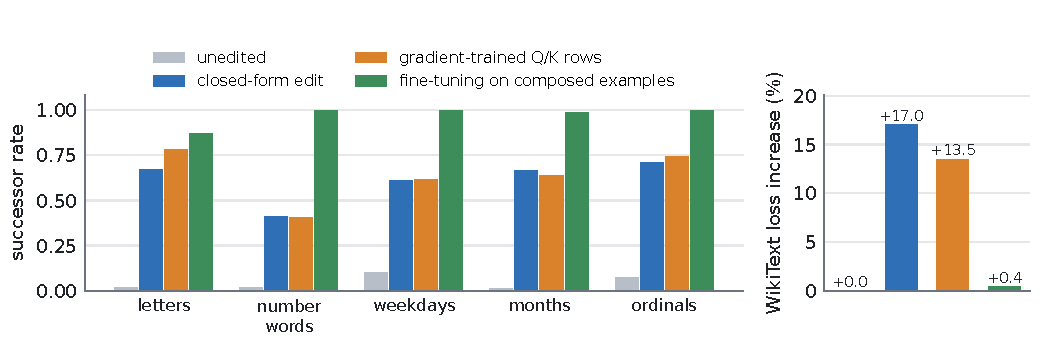
\includegraphics[width=\linewidth]{figures/learning.pdf}
\caption{Qwen3-0.6B-Base. Left: successor rate by value type for the closed-form edit, the same rows trained by gradient descent on the same routing labels (both at gain 3), and fine-tuning on examples of the composed behaviour (letters and months held out from its training). Right: increase in WikiText loss.}
\label{fig:learning}
\end{figure}

\begin{table}[t]
\centering\footnotesize
\setlength{\tabcolsep}{4pt}
\resizebox{\linewidth}{!}{\begin{tabular}{llccccccc}
\toprule
Method & Supervision & Let. & Num. & Days & Mon. & Ord. & Word lookup & WikiText \\
\midrule
Unedited & -- & .02 & .02 & .10 & .01 & .07 & .64 & +0.0\% \\
Closed-form, gain 3 & Routing labels & .67 & .41 & .61 & .66 & .71 & .54 & +17.0\% \\
Gradient Q/K, gain 3 & Routing labels & .78 & .40 & .62 & .64 & .74 & .55 & +13.5\% \\
Fine-tuning & Composed examples & .87 & 1.00 & 1.00 & .99 & 1.00 & .82 & +0.4\% \\
\bottomrule
\end{tabular}
}
\caption{Qwen3-0.6B-Base, successor rate on 300 fresh prompts per value type. Both routing methods use position labels on ordinary-word lookups. Fine-tuning updates attention projections in layers 18--24 using composed examples with number words, weekdays and ordinals; letters and months are held out. ``Word lookup'': accuracy on ordinary-word tables. ``WikiText'': relative change in loss.}
\label{tab:learning}
\end{table}

\section{Can a language model design the edit?}\label{sec:opus}

The routing edit was designed by hand, after the unsuccessful attempts of Appendix~\ref{sec:negative} in which a language model proposed low-level weight edits. Those attempts left open whether the failure lay with the editor or with the edit language. Once a working construction existed, we could ask a sharper question: given circuit-level primitives and diagnostics that show which component computes what, can a language model design an edit of this kind, and does it find anything we did not?

\subsection{Primitives and protocol}\label{sec:prims}

{\sloppy We expose the construction as four primitives that an executor applies to the weights: \texttt{attention\_program} (write a head's query rows and its key group's rows from the whitened cross-covariance of Section~\ref{sec:program}, with a choice of layer, head, the two position roles to connect, the contrast, the ridge strength, the rank and the rotary band); \texttt{copy\_qk} and \texttt{copy\_ov} (copy another head's query--key or value--output weights within a layer); and \texttt{scale\_output} (multiply a head's output projection by a gain, zero to remove it). Position roles are the query position, the queried value, the arrow before it and the queried key. A \emph{programme} is a list of at most eight primitive calls.\par}

The designer is Claude Opus 5.5. Its instructions describe the attention architecture, the task, the primitives, and diagnostics of the unedited model: the ablation ranking and oracle rates from Section~\ref{sec:locate}, the mean attention of every head to the queried value on lookup prompts, and the language-model cost of removing each head of layer 21. The designer therefore receives our closed-form construction through the documentation of the \texttt{attention\_program} primitive (the bilinear map, its factorisation and the rotary placement are described to it), but it receives no completed programme and no measurement of our hand-designed edit. In each of five rounds it returns up to three programmes with a short analysis; each programme is applied to the unedited model and measured on development data (the successor and lookup rates on one ordinal value type, ordinals; ordinary-word lookup accuracy; sequence continuation; WikiText loss; attention of the programmed heads), and the measurements are returned. By a rule fixed before the runs, the programme with the highest development successor rate among those within 15\% of the unedited WikiText loss is frozen and evaluated once on the confirmation prompts. Attention programmes inside this harness are fitted on 800 ordinary-word lookups.

\subsection{What the designer did}

We ran the protocol of Section~\ref{sec:prims} three times: twice on the 0.6B model and once, from scratch, on the 1.7B model. All three runs produced working programmes (Table~\ref{tab:opus}); each used five API calls and cost \$0.29--\$0.39.

In every run the designer's first round identified \head{21}{6} as the successor head from the diagnostics and programmed it to attend from the query position to the queried value. It then used later rounds to test hypotheses and reported the outcomes in its analyses; in the first 0.6B run, for example, it found that sharper attention does not raise the successor rate, that removing heads which copy the value does not help, and that aiming at the arrow instead of the value destroys the effect. Figure~\ref{fig:design} shows the search: early programmes are scattered, later ones concentrate near the hand-designed edit's successor rate at lower cost.

\begin{table}[t]
\centering\small
\resizebox{\linewidth}{!}{\begin{tabular}{llccccccccc}
\toprule
Model & Design & Let. & Num. & Days & Mon. & Ord. & Seq. & Word lookup & WikiText & API cost \\
\midrule
0.6B & Hand-designed & .68 & .45 & .62 & .74 & .64 & .80 & .49 & +11.4\% & -- \\
0.6B & Opus, run 1 & .54 & .45 & .60 & .61 & .58 & .90 & .53 & +7.7\% & \$0.36 \\
0.6B & Opus, run 2 & .55 & .29 & .58 & .51 & .57 & .90 & .43 & +14.5\% & \$0.39 \\
\midrule
1.7B & Hand-designed & .36 & .30 & .34 & .54 & .50 & .60 & .60 & +12.0\% & -- \\
1.7B & Opus & .28 & .27 & .57 & .65 & .59 & .60 & .59 & +7.6\% & \$0.29 \\
\bottomrule
\end{tabular}
}
\caption{Hand-designed edit and programmes written by Claude Opus, measured with the same harness (attention programmes fitted on 800 ordinary-word lookups) on the same confirmation prompts (fitted format, unseen keys, 400 per value type). Columns Let.--Ord.: successor rate. Seq.: accuracy on ten sequence-continuation prompts. WikiText: relative change in loss. Opus's programmes were selected on a development set of ordinals only.}
\label{tab:opus}
\end{table}

\begin{figure}[t]
\centering
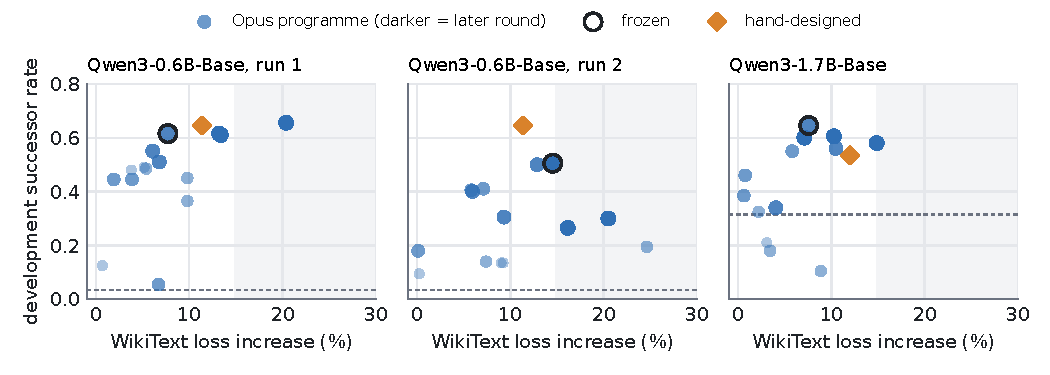
\includegraphics[width=\linewidth]{figures/design.pdf}
\caption{Every programme proposed by the designer in the three runs: development successor rate against the increase in WikiText loss. The dashed line is the unedited model; programmes in the shaded region exceed the 15\% limit and are not eligible. The hand-designed edit is measured in the same harness.}
\label{fig:design}
\end{figure}

\subsection{An unplanned design: transplanting the circuit}

The most interesting outcome was a design we had not built. Our edit has an obvious drawback: redirecting \A\ takes it away from its native job. In all three runs the designer arrived at a way around this. It copied the successor head's value--output circuit into a different head of the same layer and programmed or reused \emph{that} head's attention, so that the computation runs in a second place. The primitives allowed this, since \texttt{copy\_ov} was in the library, but the instructions list it only as one primitive among four and never suggest a transplant, and we had not tried one. Transplantation makes it possible to leave the original head alone; the second 0.6B programme does so, whereas the other two also redirect the original head. The frozen programmes differ: (0.6B, run 1) a spare head carrying the copied circuit plus the redirected original head, each at gain 1.5; (0.6B, run 2) a single spare head at gain 3.7; (1.7B) the redirected original head plus copies of its circuit into the two layer-21 heads that natively attend most to the queried value.

Is the transplanted circuit really doing the work? Table~\ref{tab:opusctl} decomposes the first 0.6B programme. Removing both programmed heads removes the effect, and removing either leaves part of it, so both heads contribute. The spare-head design alone gives 0.24--0.47, answers all ten sequence probes correctly, and raises WikiText loss by 1.9\%. These small development probes do not establish broad preservation, and we have not compared the spare-head design with lower-gain direct edits at matched successor performance. The same design with a non-successor head's circuit copied in does not reproduce the effect (at most 0.02), nor does aiming it at the arrow (at most 0.13, the unedited level for that value type), and the side effect of the copy (removing the spare head's group partner) changes nothing by itself. This table was recomputed on a GPU, whereas the first run was executed on a CPU; the refit differs slightly, so the frozen programme's row is not numerically identical to Table~\ref{tab:opus} (for example 0.53 against 0.54 on letters).

\begin{table}[t]
\centering\small
\resizebox{\linewidth}{!}{\begin{tabular}{lccccccc}
\toprule
Variant & Let. & Num. & Days & Mon. & Ord. & Seq. & WikiText \\
\midrule
Unedited & .02 & .01 & .12 & .01 & .10 & 1.00 & +0.0\% \\
Frozen programme & .53 & .46 & .60 & .62 & .58 & .90 & +7.5\% \\
\midrule
Frozen, head 0 removed & .22 & .24 & .53 & .42 & .51 & .70 & +3.9\% \\
Frozen, head 6 removed & .33 & .26 & .43 & .45 & .48 & .70 & +3.9\% \\
Frozen, all programmed heads removed & .00 & .01 & .09 & .01 & .05 & .40 & +2.1\% \\
\midrule
Spare head only: successor head's OV, aimed at the value & .39 & .24 & .45 & .46 & .47 & 1.00 & +1.9\% \\
Spare head only: head 8's OV, aimed at the value & .01 & .00 & .01 & .00 & .02 & 1.00 & +1.9\% \\
Spare head only: successor head's OV, aimed at the arrow & .04 & .02 & .13 & .01 & .09 & 1.00 & +5.8\% \\
Only the side effect (head 1 removed) & .02 & .01 & .12 & .01 & .11 & 1.00 & +0.3\% \\
\bottomrule
\end{tabular}
}
\caption{Qwen3-0.6B-Base: decomposition of the first programme designed by Opus (spare head 0 with head 6's value--output circuit, plus the redirected head 6). Successor rates on the confirmation prompts; Seq.\ and WikiText as in Table~\ref{tab:opus}.}
\label{tab:opusctl}
\end{table}

\subsection{Comparison with the hand-designed edit}

How do the designer's programmes compare with ours? Table~\ref{tab:opus} measures the hand-designed edit and the frozen programmes with the same harness, fit data and confirmation prompts. On the 0.6B model the first programme is somewhat weaker on the target behaviour (0.45--0.61 against 0.45--0.74) at two thirds of the damage to WikiText loss and with sequence continuation better preserved; the second is weaker and no cheaper. On the 1.7B model the programme is stronger than the hand-designed edit on three value types, weaker on two, at lower cost. The designs are therefore comparable to ours, not uniformly better.

\subsection{What this does and does not show}

The designer chose the component, the positions to connect, the gains, and the idea of transplanting the circuit, using the supplied diagnostics, primitive library and development feedback in all three runs. It did not invent the attention programme: that primitive encodes our construction, and a model given only raw weights and activations might not have found it. An earlier request that asked the same model to write free-form code computing the weights was declined by the API (three calls, no output); the primitive-library formulation was accepted.

Four further cautions apply. WikiText loss and sequence continuation are development measurements that the designer saw repeatedly during its search, and sequence continuation is ten prompts, so ``0.90'' means nine of ten development probes and does not establish preservation. The confirmation prompts were held out from the designer's feedback but had already been used when we developed the hand-designed edit, so they are not untouched by the research process. Three API trajectories do not establish how reliably the designer succeeds. And we have not compared it with a search of equal evaluation budget that samples programmes from the same primitives at random, so we cannot say how much of the result is due to reasoning and how much to search. The hand-designed edit in Table~\ref{tab:opus} is refitted on the harness's 800 prompts, which is why its WikiText cost there (11.4\%) differs from the 17\% of the 1{,}500-prompt fit in Section~\ref{sec:gain}.

\section{Limitations}\label{sec:limits}

The evidence covers one operation, succession, and one routing pattern, key--value lookup. The two models belong to the same family and place the selected head at the same index. Replication in an unrelated model family remains the most useful test of broader applicability. The routing fit was run once per model and format, so the prompt-level comparisons do not measure variation across fitted edits. Failures on other operations concern the six heads selected by our rule; they do not rule out other heads, interfaces or distributed implementations.

The direct edit is global. At the reported gain it increases WikiText loss by 14--17\%, disrupts native sequence continuation, and reduces ordinary-word lookup accuracy. Its successor rates remain far below reliable task performance. Gradient descent on the routing objective performs similarly, and fine-tuning on composed examples performs substantially better. We have not evaluated a simple instruction or few-shot prompting baseline for the composed task. The practical value of the edit as a way to obtain answers is therefore unestablished; the present evidence concerns understanding and controlling a computation.

The development stages use different information. Position labels on ordinary-word lookups fit the routing weights, sequence prompts locate the head, and composed-task results select the gain and the designer's programmes. Confirmation prompts are fresh relative to the direct edit's gain selection, but were reused in evaluating the designer. We report paired win/loss counts without confidence intervals across fits. The main metric checks only the first answer token, and the causal interventions establish dependence on the head's output rather than a context-independent successor function within that head alone.

Preservation measurements are limited. WikiText loss is mean token negative log-likelihood on a small fixed sample, repeatedly exposed during programme selection. The designer's sequence probes contain only ten prompts, and there is no independent preservation set or comparison at matched successor performance. The three designer runs use a library containing our routing estimator and informative diagnostics. Without equal-budget random, Bayesian or heuristic search over the same primitives, they do not establish an advantage for LLM-guided search.

\section{Discussion}

The contrast between Section~\ref{sec:results} and Appendix~\ref{sec:negative} suggests where direct weight programming has traction on models of this size. Edits that tried to improve a diffuse behaviour, or to install a mapping item by item, either did nothing beyond noise or fitted the items they were built from. The edit that worked changed only \emph{where} an existing, well-localised computation reads, and the map it needed could be estimated from data that share the routing structure but not the content. Our failed self-composition attempts point the same way: we found a useful linear input interface but no output bridge that generalised convincingly in the tested settings.

A similar contrast appears for the language model as editor. Asked to improve reasoning efficiency with low-level rank-one writes, it produced no clear validation gain; given diagnostics that expose which component computes what, and primitives that act on whole circuits, all three runs produced working programmes within five rounds. Task, supervision, diagnostics, primitives and evaluation all differ between those studies, so they do not isolate the level of abstraction of the edit language as the cause; they motivate a controlled comparison of editing abstractions.

Taken together, these results suggest a different picture of what programming a pretrained network might involve. The unit of editing in our successful experiments was not a weight or a rank-one direction but a circuit with a known role: locate a computation, re-aim its input, copy it elsewhere, scale its vote. At that level, the hard part of the problem moves. Writing the new weights was a ridge regression. Finding a computation whose input could be separated from its function was the difficult step, and it succeeded for only one of the five operations we tried: succession passed our locating rule, while capitalisation, pluralisation, past tense and antonyms did not. The transplant designs add a second possibility. If a computation can be copied into another head, reusing it need not take it away from its original role, although our evidence for preservation is limited to a small development sample.

The practical case for routing edits is not yet made. Fine-tuning on composed examples is more accurate and less damaging, and we have not compared against prompting. The strongest use of the edit today is as an intervention: it tests whether a located computation can be reused after changing its source of input, and for succession the answer is yes.

The question this leaves is not ``can an editor improve a model?'', which is too broad to answer, but: which computations in a pretrained model have input interfaces that can be re-aimed, and what is the cheapest supervision that re-aims them? A survey over many operations and model families, with the locating rule fixed in advance and the failures reported, would show whether succession is an isolated case or one example of a larger set of reusable parts.

\sloppy
\section*{Reproducibility}
\begingroup\raggedright
Code, prompt generators, result files and logs are archived in the project repository: \url{https://github.com/Richard-Y-W/Machine-learning-research-paper}. The routing experiments are in \texttt{experiments/compose/}; earlier studies are in \texttt{experiments/amortize/}, \texttt{experiments/evolution/} and \texttt{experiments/skill/}. Tables and figures are generated from saved results by \texttt{paper/make\_tables.py} and \texttt{paper/make\_figures.py}. The closed-form construction uses forward passes and linear algebra; the learning comparisons also use gradient training. The designer runs used the Anthropic API.

The lookup fit uses Python's random seed string \texttt{lookup-v3}; confirmation uses \texttt{confirm-v1|} followed by the format label in \texttt{lookup3\_confirm.py}. The digit experiment uses \texttt{increment-v1}, the learning comparison \texttt{learning-cmp-v1}, and the designer harness \texttt{opus-program-v1}. Value and key lists, exclusions, and tokenisation rules are defined in the corresponding generators. Model loading uses float32 weights from \texttt{Qwen/Qwen3-0.6B-Base} or \texttt{Qwen/Qwen3-1.7B-Base}. The original loader does not pin a checkpoint revision, so exact run-specific revisions cannot be established from its records alone.

WikiText measurements use the \texttt{wiki\_dev} token arrays archived in \texttt{results/evolution/splits.json}: four chunks of 128 tokens from WikiText-103-raw-v1's test split. Loss averages the 127 next-token predictions within each chunk (508 predictions in total), with no prediction across chunk boundaries. The relative change is $100(\mathrm{NLL}_{\mathrm{edited}}/\mathrm{NLL}_{\mathrm{base}}-1)$. This sample is reused during development and is not an independent confirmation of preservation. The appendix summarises the remaining evaluation sets.
\par\endgroup

\section*{Acknowledgements}
AI assistants (Claude and Codex) were used for coding and editing.

\begin{thebibliography}{99}\small\raggedright
\bibitem{sparks} R.~Takehi, J.~Teoh, A.~Zhang, and O.~Khattab. Sparks of weight-space programming. MIT CSAIL, blog post, November 2026. \url{https://rikiyat.github.io/blog/weight-space-programming/}.
\bibitem{hu2026wsp} J.~Hu, C.~Tang, W.~Li, H.~Zhu, C.-M.~Feng, Q.~Zhang, Y.~Chen, and M.~Hu. Exploring weight-space programming: Capabilities, generalization, and limitations. arXiv:2611.09382, 2026.
\bibitem{wspscratch} C.~Singh. Weight-space programming from scratch on simple tasks. Web report, November 2, 2026. \url{https://csinva.io/weight-space-programming-autoresearch/analyze/toy_examples/report.html}.
\bibitem{mbe2024} J.~Singh, S.~Dutta, and T.~Chakraborty. Mechanistic behavior editing of language models. arXiv:2410.04277, 2024.
\bibitem{tiwari2026qk} K.~Tiwari, V.~Chordia, and Prathosh A.~P. Spectral query-key product weight steering for training-free VLM hallucination mitigation. arXiv:2606.20419, 2026.
\bibitem{gould2023successor} R.~Gould, E.~Ong, G.~Ogden, and A.~Conmy. Successor heads: Recurring, interpretable attention heads in the wild. arXiv:2312.09230, 2023.
\bibitem{qwen3} A.~Yang, A.~Li, B.~Yang, et al. Qwen3 technical report. arXiv:2505.09388, 2025.
\bibitem{elhage2021framework} N.~Elhage, N.~Nanda, C.~Olsson, et al. A mathematical framework for transformer circuits. Transformer Circuits Thread, 2021.
\bibitem{olsson2022induction} C.~Olsson, N.~Elhage, N.~Nanda, et al. In-context learning and induction heads. Transformer Circuits Thread, 2022.
\bibitem{wang2023ioi} K.~Wang, A.~Variengien, A.~Conmy, B.~Shlegeris, and J.~Steinhardt. Interpretability in the wild: A circuit for indirect object identification in GPT-2 small. ICLR, 2023.
\bibitem{merullo2024reuse} J.~Merullo, C.~Eickhoff, and E.~Pavlick. Circuit component reuse across tasks in transformer language models. ICLR, 2024.
\bibitem{todd2024function} E.~Todd, M.~L.~Li, A.~S.~Sharma, A.~Mueller, B.~C.~Wallace, and D.~Bau. Function vectors in large language models. ICLR, 2024.
\bibitem{meng2022rome} K.~Meng, D.~Bau, A.~Andonian, and Y.~Belinkov. Locating and editing factual associations in GPT. NeurIPS, 2022.
\bibitem{meng2023memit} K.~Meng, A.~S.~Sharma, A.~Andonian, Y.~Belinkov, and D.~Bau. Mass-editing memory in a transformer. ICLR, 2023.
\bibitem{belrose2023tuned} N.~Belrose, Z.~Furman, L.~Smith, et al. Eliciting latent predictions from transformers with the tuned lens. arXiv:2303.08112, 2023.
\bibitem{ilharco2023task} G.~Ilharco, M.~T.~Ribeiro, M.~Wortsman, et al. Editing models with task arithmetic. ICLR, 2023.
\bibitem{hu2022lora} E.~J.~Hu, Y.~Shen, P.~Wallis, et al. LoRA: Low-rank adaptation of large language models. ICLR, 2022.
\bibitem{lindner2023tracr} D.~Lindner, J.~Kram\'ar, S.~Farquhar, M.~Rahtz, T.~McGrath, and V.~Mikulik. Tracr: Compiled transformers as a laboratory for interpretability. NeurIPS, 2023.
\bibitem{ainslie2023gqa} J.~Ainslie, J.~Lee-Thorp, M.~de~Jong, Y.~Zemlyanskiy, F.~Lebr\'on, and S.~Sanghai. GQA: Training generalized multi-query transformer models from multi-head checkpoints. EMNLP, 2023.
\bibitem{su2021roformer} J.~Su, Y.~Lu, S.~Pan, A.~Murtadha, B.~Wen, and Y.~Liu. RoFormer: Enhanced transformer with rotary position embedding. arXiv:2104.09864, 2021.
\end{thebibliography}

\appendix
\section{Earlier experiments and unsuccessful constructions}\label{sec:negative}

\textbf{Iterative edits proposed by a language model.} Before the routing edit we ran three studies in which Claude Opus proposed weight edits in a small edit language (rank-one writes and scalings built from singular vectors, token embeddings and mean activations), with selection on held-out data. (i)~In an evolutionary search on multiple-choice benchmarks, lineages of model-proposed edits did not outperform lineages of random edits of matched size or a small evolution strategy; all bootstrap intervals on the contrasts included zero, and unions of edits from two lineages lost accuracy. (ii)~Edits meant to install a new letter-shift skill fitted practice items and scored zero on held-out items; an affine answer-writing map behaved the same way. (iii)~In the chat model Qwen3-0.6B we tried to reduce the reasoning tokens needed to trace short Python programs. A single prompt sentence (``Keep your thinking under 100 words.'') raised accuracy within 256 generated tokens from about 0.05--0.10 to about 0.40; end-of-thinking logit bias, steering vectors and random edits did not establish an improvement. Combining the short-answer prompt with forced stopping reached 0.52 at 256 tokens, but reduced longer-budget accuracy to about 0.57. With selection run under that prompt, paired scoring and a strict acceptance rule, seven rounds of proposals yielded one accepted edit and no measurable validation gain (0.400 to 0.417 on 60 items; 0.30 to 0.23 on the held-out program family). Every proposal targeted the same thing, a direction associated with re-checking.

\textbf{Applying the successor head twice.} We tried to make the model skip two items in a native sequence by feeding \A's output back into a successor computation. A ridge map into a later head, fitted on non-letter sequences, gave two-step answers on at most 9\% of letter prompts as a weight edit. A linear ``shift'' in \A's output space reached 0.89 on the sequences it was fitted on and 0.01--0.06 on letters; fitted on twelve letters it scored 0.00 on eight others. Read through the unembedding, \A's output has the next item as top-1 in 0\% of letter prompts: it is an intermediate code that later layers decode. An item-agnostic map from unembedding rows to layer-21 inputs, fitted on 5{,}400 ordinary words, is a valid \emph{input} interface (two-step rate 0.91 when it is handed the true next token) and raised the two-step rate to 0.29 on letters and 0.46 on other sequences when fed \A's own output; this last number has no matched random control and we do not interpret it.

\textbf{Other routes to the lookup composition.} Rewriting the output projections of heads involved in retrieval so that they write \A's code did no better than a shuffled-pairing control. Copying the query and key weights of an existing same-layer head that attends to the value did no better than copying those of a head that does not; native retrieval attention is diffuse (at most 0.38 on the queried value).

\textbf{A second operation.} The locating rule requires an operation the model performs natively with the item as the final token. With three demonstrations, Qwen3-0.6B-Base performs capitalisation, pluralisation, past tense and antonyms at only 0.42--0.60 in that format; with eight demonstrations both models reach 0.79--1.00. Applying the locating rule to the 0.6B model with eight demonstrations, capitalisation, pluralisation and past tense pass the competence gate (0.90--1.00) but fail the oracle step: for each of the six heads whose removal hurts most, substituting the head's value vector from a prompt ending in a different item never moves the answer to the operation applied to that item (0.00 in all eighteen cases), while the model often still answers correctly for its own item. Antonyms fall just below the competence gate. On the 1.7B model all four operations pass the competence gate (0.81--1.00) and all four fail the oracle step in the same way (0.00 in all twenty-four cases). For these operations, then, none of the six heads selected by our rule passed the oracle intervention. This does not exclude other heads, other interfaces or distributed implementations, but the recipe as stated does not apply to them; succession is the only operation for which it has been demonstrated.


\section{Programmes frozen by the language-model designer}\label{app:programmes}

Each programme is listed as the sequence of primitive calls returned by the designer, in the order applied to the unedited weights. The full instructions given to the designer, every programme it proposed, its analyses, and the measurements returned to it are in the repository under \texttt{results/compose*/opus\_program/}.

\paragraph{Qwen3-0.6B-Base, run 1.} Frozen in round 4 of 5 (15 programmes evaluated). Development successor rate 0.61 (unedited 0.04).
\begin{Verbatim}[fontsize=\scriptsize,breaklines=true,breakanywhere=true]
{"op": "attention_program", "layer": 21, "head": 0, "query_role": "final", "key_role": "queried_value", "contrast": "other_positions", "ridge": 1.0, "rank": 32, "rope_band": "low"}
{"op": "copy_ov", "layer": 21, "from_head": 6, "to_head": 0}
{"op": "scale_output", "layer": 21, "head": 1, "gain": 0.0}
{"op": "scale_output", "layer": 21, "head": 0, "gain": 1.5}
{"op": "attention_program", "layer": 21, "head": 6, "query_role": "final", "key_role": "queried_value", "contrast": "other_values", "ridge": 1.0, "rank": 32, "rope_band": "low"}
{"op": "scale_output", "layer": 21, "head": 6, "gain": 1.5}
\end{Verbatim}
\paragraph{Qwen3-0.6B-Base, run 2.} Frozen in round 5 of 5 (15 programmes evaluated). Development successor rate 0.51 (unedited 0.04).
\begin{Verbatim}[fontsize=\scriptsize,breaklines=true,breakanywhere=true]
{"op": "attention_program", "layer": 21, "head": 5, "query_role": "final", "key_role": "queried_value", "contrast": "other_positions", "ridge": 1.0, "rank": 16, "rope_band": "low"}
{"op": "copy_ov", "layer": 21, "from_head": 6, "to_head": 5}
{"op": "scale_output", "layer": 21, "head": 4, "gain": 0.0}
{"op": "scale_output", "layer": 21, "head": 5, "gain": 3.7}
\end{Verbatim}
\paragraph{Qwen3-1.7B-Base.} Frozen in round 4 of 5 (13 programmes evaluated). Development successor rate 0.65 (unedited 0.32).
\begin{Verbatim}[fontsize=\scriptsize,breaklines=true,breakanywhere=true]
{"op": "attention_program", "layer": 21, "head": 6, "query_role": "final", "key_role": "queried_value", "contrast": "other_values", "ridge": 3.0, "rank": 16, "rope_band": "low"}
{"op": "scale_output", "layer": 21, "head": 6, "gain": 1.5}
{"op": "copy_ov", "layer": 21, "from_head": 6, "to_head": 8}
{"op": "copy_ov", "layer": 21, "from_head": 6, "to_head": 15}
{"op": "scale_output", "layer": 21, "head": 8, "gain": 2.0}
{"op": "scale_output", "layer": 21, "head": 15, "gain": 2.0}
\end{Verbatim}


\section{Summary of evaluation sets}

\begin{itemize}
\item \emph{Fitting} (hand-designed edit): 1{,}500 lookup prompts with ordinary-word values in the $k \rightarrow v$ format; 200 further ordinary-word prompts, of which the first 100 choose $\lambda$. Inside the designer harness: 800 prompts.
\item \emph{First evaluation} (0.6B only; used to choose the gain): 300 prompts per value type.
\item \emph{Confirmation}: 400 prompts per value type and format, generated after the gain was frozen, with thirty key words disjoint from those used in fitting. The designer's programmes are evaluated on the same prompts.
\item \emph{Designer development set}: 200 lookup prompts with ordinal-word values, 150 ordinary-word lookups, ten sequence prompts, and a fixed WikiText sample.
\item \emph{Controls}: 300 fresh prompts per value type (Tables~\ref{tab:controls} and~\ref{tab:cf}); the confirmation prompts (Table~\ref{tab:opusctl}).
\end{itemize}

\end{document}
